\chapter{Chimie bioinorganique}\label{ch:b3:bioinorganic}

Notre sang est rouge à cause du fer~; le sang d'une limule est incolore dans
ses veines et bleuit à l'air, parce qu'il transporte le dioxygène sur du
cuivre. Le vivant utilise une poignée d'ions métalliques pour les tâches
qu'aucun groupe organique ne sait accomplir~: fixer le dioxygène de façon
réversible, transporter des électrons un par un, couper l'eau, réduire le
diazote, rendre une molécule d'eau assez acide pour attaquer le dioxyde de
carbone. Ce chapitre lit ces tâches avec les outils de la chimie de
coordination~: \omterm{def:b3:bioinorganic:hsab}{acides durs} et mous, champ des ligands et états de spin,
équilibres et lois de vitesse, et il se termine par les métaux utilisés
comme médicaments.

\begin{recall}
Le volume de deuxième année a traité des acides $\alpha$-aminés, des chaînes latérales et des peptides,
des bases nucléiques et des nucléotides, des complexes de coordination, du
champ des ligands, des états haut spin et bas spin, et des nucléophiles et
électrophiles durs et mous~; le volume de première année, des constantes de
complexation et de l'échelle de pL. Le
\cref{ch:b3:complex-spectra-magnetism} et le \cref{ch:b3:complex-mechanisms}
ont donné les spectres, la théorie de Marcus et l'aquation du cisplatine, le
\cref{ch:b3:complex-kinetics} la cinétique de Michaelis--Menten, et le
\cref{ch:b3:advanced-nmr} le temps de relaxation $T_1$.
\end{recall}

\begin{omfigure}
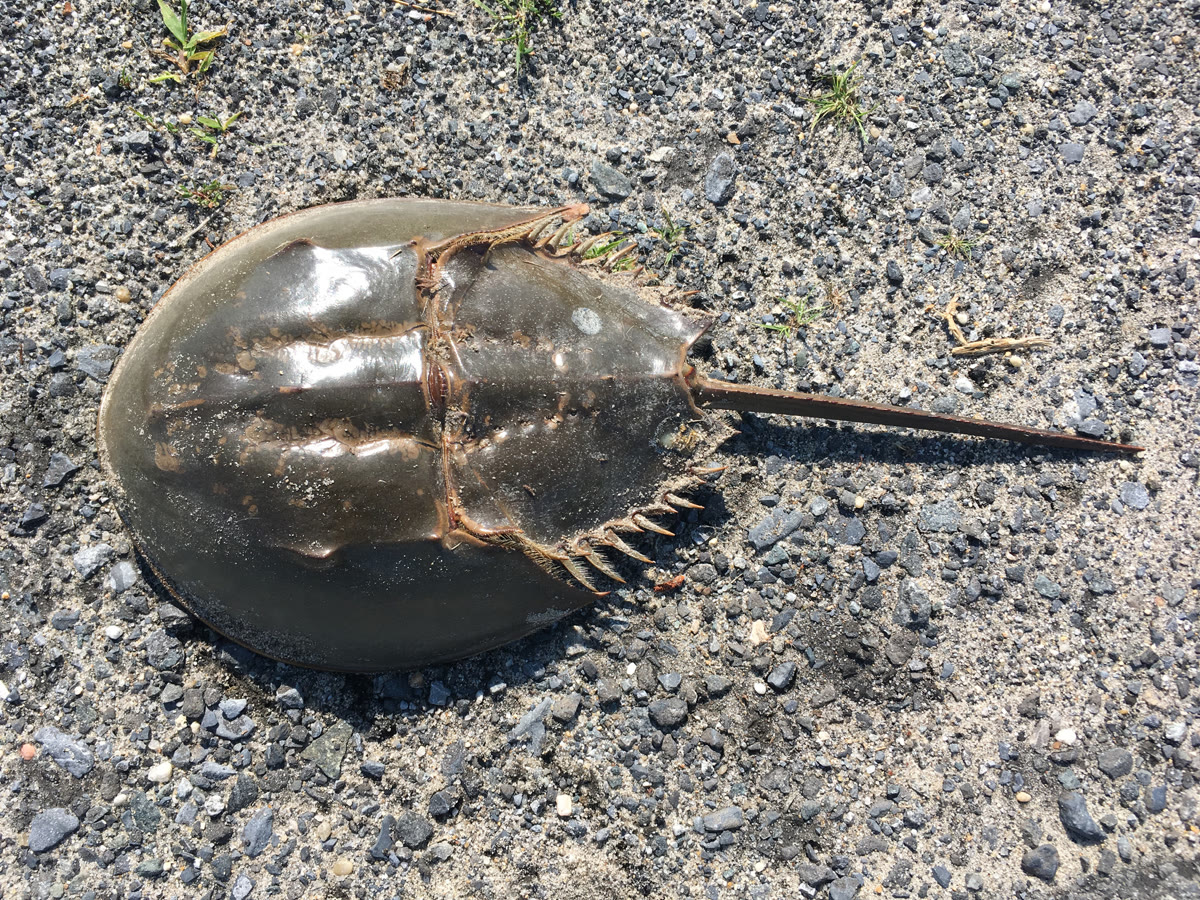
\includegraphics[width=0.5\linewidth]{images/book4/horseshoe-crab.jpg}

{\small Une limule de l'Atlantique. Son sang transporte le dioxygène sur
l'hémocyanine, une protéine à cuivre, et il est bleu lorsqu'il est oxygéné.
Photographie~: Kaldari, CC0.}
\end{omfigure}

\section{Les métaux en biologie}

\begin{definition}[Métalloprotéines]\label{def:b3:bioinorganic:metalloprotein}
Une \emph{métalloprotéine}\index{metalloproteine@métalloprotéine} est une protéine qui contient
des ions métalliques liés~; une \emph{métalloenzyme}\index{metalloenzyme@métalloenzyme} est une
métalloprotéine qui catalyse une réaction. Un \emph{cofacteur}\index{cofacteur} est une espèce non protéique,
ion métallique ou petite molécule, liée à une protéine et nécessaire à son
activité.
\end{definition}

Les métaux présents en quantité sont le sodium, le potassium, le magnésium
et le calcium, qui portent surtout des charges et maintiennent des
structures~; les métaux de transition fer, zinc, cuivre, manganèse, cobalt,
molybdène et nickel n'existent qu'à l'état de traces mais assurent une
grande partie de la chimie. Une protéine choisit son métal par les atomes
donneurs qu'elle offre et par leur géométrie.

\begin{definition}[Acides durs et mous]\label{def:b3:bioinorganic:hsab}
Un \emph{acide dur}\index{acide dur} est un acide de Lewis petit, très chargé et peu
polarisable ($\ce{H+}$, $\ce{Mg^2+}$, $\ce{Ca^2+}$, $\ce{Fe^3+}$)~; un \emph{acide mou}\index{acide mou} est un acide
gros, polarisable et peu chargé ($\ce{Cu+}$, $\ce{Ag+}$,
$\ce{Hg^2+}$, $\ce{Cd^2+}$). Le \emph{principe des acides et des bases durs et mous}\index{principe des acides et des bases durs et mous}
énonce que les acides durs se lient de préférence aux bases dures (donneurs
oxygénés, fluorure) et les acides mous aux bases molles (donneurs soufrés,
iodure).
\end{definition}

Dans les protéines, les carboxylates et les phénolates sont durs, le
thiolate de la cystéine et le thioéther de la méthionine mous, et
l'imidazole de l'histidine intermédiaire. Le fer(III) se place parmi des
donneurs oxygénés, le cuivre(I) parmi des donneurs soufrés, le zinc, acide
intermédiaire, avec l'histidine et la cystéine~; le mercure et le cadmium
sont toxiques en partie parce qu'ils s'emparent des cystéines des \omterm{def:b3:complex-kinetics:enzyme}{enzymes}.

\begin{definition}[Série d'Irving--Williams]\label{def:b3:bioinorganic:irving-williams}
La \emph{série d'Irving--Williams}\index{serie d'Irving--Williams@série d'Irving--Williams} est l'ordre de stabilité
des complexes haut spin des ions divalents de la première série de
transition avec un ligand donné~:
$\ce{Mn^2+} < \ce{Fe^2+} < \ce{Co^2+} < \ce{Ni^2+} < \ce{Cu^2+} > \ce{Zn^2+}$.
\end{definition}

\begin{proposition}[Ordre d'Irving--Williams]\label{prop:b3:bioinorganic:irving-williams}
La série est vérifiée pour presque tous les ligands (c'est une observation
expérimentale)~; elle suit la diminution du rayon ionique du manganèse au
cuivre, l'énergie de stabilisation du champ des ligands, nulle pour $d^5$, maximale pour $d^8$, et la
distorsion de Jahn--Teller du cuivre(II), qui raccourcit quatre de ses
liaisons.
\end{proposition}

\begin{proof}[Justification]
Le rayon diminue le long de la période à mesure que la charge nucléaire
augmente, ce qui renforce l'attraction électrostatique de chaque ligand. La
stabilisation du champ des ligands des ions octaédriques haut spin
(\cref{ch:b3:complex-spectra-magnetism}) vaut $0$, $4$,
$8$, $12$ et $6\,\mathrm{Dq}$ pour $d^5$ à $d^9$, et $0$ pour $d^{10}$~: elle renforce la tendance jusqu'au nickel et
s'effondre pour le zinc~; le cuivre(II) regagne, par sa distorsion
tétragonale, plus que ne le suggère sa stabilisation, car elle lui donne
quatre liaisons courtes et fortes.
\end{proof}

Une conséquence que les cellules doivent gérer~: le cuivre et le zinc
supplanteraient les autres ions dans la plupart des sites, si bien que
leurs concentrations libres sont maintenues extrêmement basses par des
protéines de transport dédiées.

\section{Le transport du dioxygène}

\begin{definition}[Porphyrines et hème]\label{def:b3:bioinorganic:haem}
Une \emph{porphyrine}\index{porphyrine} est un grand macrocycle plan et
aromatique formé de quatre cycles pyrrole reliés par des ponts méthine, dont
les quatre azotes lient un ion métallique en son centre. L'\emph{hème}\index{heme@hème}
est le complexe du fer de la protoporphyrine~IX, \omterm{def:b3:bioinorganic:metalloprotein}{cofacteur} de l'hémoglobine,
de la myoglobine et des cytochromes.
\end{definition}

Dans la myoglobine et l'hémoglobine, le fer de l'\omterm{def:b3:bioinorganic:haem}{hème} porte un cinquième
ligand sous le cycle, l'azote de l'histidine proximale, et un sixième site
libre pour $\ce{O2}$. Le fer(II) de la forme désoxy est haut spin~: un électron dans l'orbitale $d_{x^2-y^2}$, qui pointe vers les quatre
azotes, le rend trop gros pour la cavité du cycle, et il se place hors du
plan, du côté de l'histidine. En fixant $\ce{O2}$, il devient bas spin, plus petit, et
se déplace dans le plan, entraînant avec lui l'histidine et l'hélice de la
protéine.

\begin{omfigure}
% ledger: pdb:Hb.deoxy.FeN4, pdb:Hb.oxy.FeN4
\begin{tikzpicture}[font=\small, scale=0.9]
  \foreach \x/\lab/\dz/\oxy in {0/désoxy (haut spin)/-0.34/0, 6.4/oxy (bas spin)/-0.04/1} {
    \begin{scope}[xshift=\x cm]
      \draw[omDef, line width=2.6pt] (-2.2,0) -- (2.2,0);
      \node[font=\scriptsize, anchor=west, omDef] at (2.3,0) {porphyrine};
      \fill[omThm] (0,\dz*1.5) circle (0.22);
      \node[font=\scriptsize, anchor=north west] at (0.2,\dz*1.5-0.12) {Fe};
      \draw[black!70, line width=1pt] (0,\dz*1.5-0.22) -- (0,-1.55);
      \node[draw=black!70, regular polygon, regular polygon sides=5, minimum size=7mm, inner sep=0pt] at (0,-1.95) {};
      \node[font=\scriptsize, anchor=west] at (0.45,-1.95) {His proximale};
      \node[font=\small\bfseries] at (0,1.9) {\lab};
      \ifnum\oxy=1
        \draw[black!70, line width=1pt] (0,0.2) -- (0,0.85) -- (0.55,1.25);
        \fill[red!75] (0,0.85) circle (0.13) (0.55,1.25) circle (0.13);
        \node[font=\scriptsize, anchor=west] at (0.75,1.2) {$\ce{O2}$, coudé};
      \fi
    \end{scope}
  }
  \draw[<->, black!60] (-1.0,0) -- (-1.0,-0.51) node[midway, left, font=\scriptsize] {\qty{0.34}{\angstrom}};
\end{tikzpicture}

{\small Le fer de l'\omterm{def:b3:bioinorganic:haem}{hème} vu par la tranche, son déplacement par rapport au
cycle étant dessiné à l'échelle (1~\AA{} pour 1.35~cm~; les autres distances sont schématiques). Dans la désoxyhémoglobine, le fer(II) haut spin se trouve
\qty{0.34}{\angstrom} sous le plan moyen des quatre azotes pyrroliques, du
côté de l'histidine proximale~; dans l'oxyhémoglobine, il est à moins de \qty{0.05}{\angstrom} du plan, avec $\ce{O2}$
lié par une extrémité et coudé (distances calculées à partir de structures
cristallines).}
\end{omfigure}

Le dioxygène lié est mieux décrit comme un superoxyde sur un fer(III), $\ce{Fe^{III}-O2^-}$, que comme
un $\ce{O2}$ neutre sur un fer(II)~: le complexe est diamagnétique parce que les électrons non
appariés des deux centres se couplent. La protéine empêche l'oxydation
irréversible en fer(III) et en eau, que subit immédiatement un \omterm{def:b3:bioinorganic:haem}{hème} nu dans
l'eau.

\begin{definition}[Fixation coopérative]\label{def:b3:bioinorganic:cooperativity}
La fixation sur une protéine à plusieurs sites est \emph{coopérative}\index{fixation cooperative@fixation coopérative}
lorsque la fixation d'un ligand augmente l'affinité des sites restants. Le
\emph{coefficient de Hill}\index{coefficient de Hill} $n$ est la pente du
diagramme de Hill, $\log\frac{\theta}{1 - \theta}$ en fonction de $\log p$, à demi-saturation ($\theta$ est la fraction des sites
occupés).
\end{definition}

\begin{proposition}[Un seul site]\label{prop:b3:bioinorganic:hyperbola}
Pour une protéine à un seul site, $\mathrm{P + O_2 \rightleftharpoons PO_2}$, la fraction occupée vaut $\theta = p/(p_{50} + p)$, où $p_{50}$ est
la constante de dissociation exprimée comme une pression.
\end{proposition}

\begin{proof}
$K_d = [\mathrm P]p/[\mathrm{PO_2}] = p_{50}$, donc $[\mathrm{PO_2}] = [\mathrm P]p/p_{50}$, et $\theta = [\mathrm{PO_2}]/([\mathrm P] + [\mathrm{PO_2}]) = (p/p_{50})/(1 + p/p_{50})$.
\end{proof}

\begin{theorem}[Équation de Hill]\label{thm:b3:bioinorganic:hill}
Pour une protéine à $n$ sites qui sont soit tous vides, soit tous occupés,
$\mathrm{P + n\,O_2 \rightleftharpoons P(O_2)_n}$,
\[
  \theta = \frac{p^n}{p_{50}^n + p^n}, \qquad \log\frac{\theta}{1 - \theta} = n\log p - n\log p_{50}.
\]
\end{theorem}

\begin{proof}
$K_d = [\mathrm P]p^n/[\mathrm{P(O_2)_n}]$~; posons $K_d = p_{50}^n$. La fraction des sites occupés est celle des molécules
sous forme remplie, $\theta = [\mathrm{P(O_2)_n}]/([\mathrm P] + [\mathrm{P(O_2)_n}]) = (p/p_{50})^n/(1 + (p/p_{50})^n)$. Alors $\theta/(1 - \theta) = (p/p_{50})^n$, et le passage
aux logarithmes donne la droite de pente $n$.
\end{proof}

L'hémoglobine, à quatre sites, n'est pas totalement \omterm{def:b3:bioinorganic:cooperativity}{coopérative}~: son
\omterm{def:b3:bioinorganic:cooperativity}{coefficient de Hill} est nettement inférieur à 4, environ 3, et son
diagramme de Hill a une pente de 1 aux deux extrémités, où elle se comporte
comme une protéine désoxy ou oxy à sites indépendants. La coopérativité
vient d'un changement de structure quaternaire~: le mouvement du fer dans
le plan du premier \omterm{def:b3:bioinorganic:haem}{hème} qui fixe $\ce{O2}$ est transmis aux autres sous-unités.

\begin{omfigure}
\begin{tikzpicture}
\begin{axis}[name=a, width=0.48\linewidth, height=5.6cm, xmin=0, xmax=14, ymin=0, ymax=1.02,
  axis lines=left, xlabel={$p(\ce{O2})$ / \unit{kPa}}, ylabel={saturation $\theta$},
  tick label style={font=\scriptsize}, label style={font=\small}]
\addplot[omMeth, thick] table[x=p, y=Mb] {figdata/out/bachelor-3-oxygen-binding.dat};
\addplot[omThm, thick] table[x=p, y=Hb] {figdata/out/bachelor-3-oxygen-binding.dat};
\addplot[omThm, thick, dashed] table[x=p, y=Hbacid] {figdata/out/bachelor-3-oxygen-binding.dat};
\draw[black!35] (axis cs:5,0) -- (axis cs:5,1.0) (axis cs:13,0) -- (axis cs:13,1.0);
\node[font=\scriptsize, anchor=south] at (axis cs:5,0.02) {tissus};
\node[font=\scriptsize, anchor=south east] at (axis cs:13,0.02) {poumons};
\node[font=\scriptsize, omMeth] at (axis cs:1.9,0.96) {Mb};
\node[font=\scriptsize, omThm] at (axis cs:7.5,0.6) {Hb};
\end{axis}
\begin{axis}[at={(a.east)}, anchor=west, xshift=1.4cm, width=0.48\linewidth, height=5.6cm,
  xmin=-1.5, xmax=1.5, ymin=-3, ymax=3, axis lines=left,
  xlabel={$\log_{10}(p/\unit{kPa})$}, ylabel={$\log_{10}\bigl(\theta/(1-\theta)\bigr)$},
  tick label style={font=\scriptsize}, label style={font=\small}]
\draw[black!30] (axis cs:-1.5,0) -- (axis cs:1.5,0);
\addplot[omMeth, thick] table[x=lgp, y=Mb] {figdata/out/bachelor-3-oxygen-binding-b.dat};
\addplot[omThm, thick, restrict y to domain=-3:3] table[x=lgp, y=Hb] {figdata/out/bachelor-3-oxygen-binding-b.dat};
\node[font=\scriptsize, omMeth, anchor=west] at (axis cs:-1.1,1.4) {pente 1};
\node[font=\scriptsize, omThm, anchor=west] at (axis cs:0.75,-1.5) {pente 2.7};
\end{axis}
\end{tikzpicture}

{\small À gauche~: saturation en dioxygène de la myoglobine (en vert) et de
l'hémoglobine (en rouge~; en tirets~: à pH plus bas) en fonction de la
pression de dioxygène, avec les valeurs du modèle
$p_{50} = \qty{0.37}{kPa}$ (Mb) et \qty{3.5}{kPa} (Hb), $n = 2.7$. Entre les poumons et les tissus, l'hémoglobine
cède un quart de son dioxygène, la myoglobine presque rien. À droite~: les
diagrammes de Hill correspondants, des droites dans ce modèle (le diagramme
de l'hémoglobine réelle s'infléchit vers une pente de 1 aux deux
extrémités).}
\end{omfigure}

\begin{method}[Lire un diagramme de Hill]\label{met:b3:bioinorganic:hill-plot}
\begin{enumerate}
  \item À partir de chaque saturation mesurée, calculer $\log(\theta/(1 - \theta))$~; la tracer en fonction de $\log p$.
  \item La pression où le tracé coupe zéro est $p_{50}$.
  \item La pente en ce point est le \omterm{def:b3:bioinorganic:cooperativity}{coefficient de Hill}~: $n = 1$ signifie des sites
        indépendants, $n > 1$ une \omterm{def:b3:bioinorganic:cooperativity}{fixation coopérative}.
  \item Avec deux points seulement, $n = \Delta\log(\theta/(1 - \theta))/\Delta\log p$.
\end{enumerate}
\end{method}

L'hémoglobine fixe aussi des protons et du dioxyde de carbone sur des sites
éloignés de l'\omterm{def:b3:bioinorganic:haem}{hème}, ce qui décale sa courbe vers la droite là où ils
abondent, dans les tissus actifs~: l'effet Bohr libère davantage de
dioxygène exactement là où il est nécessaire.

\begin{proposition}[Compétition du monoxyde de carbone]\label{prop:b3:bioinorganic:haldane}
Si le monoxyde de carbone et le dioxygène se disputent les mêmes sites, avec
$\mathrm{HbO_2 + CO \rightleftharpoons HbCO + O_2}$ de constante d'équilibre $M$, alors
$[\mathrm{HbCO}]/[\mathrm{HbO_2}] = M\,p(\ce{CO})/p(\ce{O2})$.
\end{proposition}

\begin{proof}
À l'équilibre, $M = [\mathrm{HbCO}]\,p(\ce{O2})/([\mathrm{HbO_2}]\,p(\ce{CO}))$~; un réarrangement donne le résultat.
\end{proof}

$M$ vaut quelques centaines pour l'hémoglobine humaine, si bien que
quelques centaines de parties par million de monoxyde de carbone occupent
une grande fraction des sites~; pire, les sites restés libres retiennent
plus fortement leur dioxygène, car la coopérativité agit sur eux. L'\omterm{def:b3:bioinorganic:haem}{hème}
libre fixe le monoxyde de carbone bien plus fortement encore~: dans la
protéine, une histidine distale située au-dessus du fer gêne la géométrie
linéaire Fe--C--O que préfère le monoxyde de carbone, tandis qu'elle forme une liaison hydrogène avec le
$\ce{O2}$ coudé. D'autres animaux utilisent d'autres métaux~: les hémocyanines des mollusques et des arthropodes
fixent $\ce{O2}$ entre deux ions cuivre sous forme de peroxyde, les hémérythrines de certains
vers marins sur une paire d'ions fer.

\begin{inthelab}[Une courbe de fixation du dioxygène]
Une solution d'hémoglobine en tampon est placée dans une cuve étanche aux
gaz munie d'un ballon latéral. On la débarrasse d'abord du dioxygène par un
balayage de diazote, puis on injecte des volumes connus d'air et on
équilibre la solution en l'inclinant doucement. Après chaque ajout, on
enregistre le spectre visible~: les bandes de la forme désoxy (une bande vers \qty{555}{nm}) cèdent la place aux deux bandes de la forme oxy,
et la saturation se lit sur l'absorbance à une longueur d'onde, entre ses
limites désoxy et oxy.
\end{inthelab}

\section{Métalloenzymes}

L'anhydrase carbonique accélère $\ce{CO2 + H2O <=> HCO3- + H+}$, qui prend quelques secondes dans l'eau
seule, ce qui compte lors du bref passage du globule rouge dans un
capillaire pulmonaire. Son ion zinc est tenu par trois histidines et une
molécule d'eau. Petit cation très chargé, il abaisse le $\mathrm pK_a$ de cette eau d'environ 14 à
environ 7~: au pH physiologique, une bonne partie de l'\omterm{def:b3:complex-kinetics:enzyme}{enzyme} porte un
hydroxyde lié au zinc, nucléophile puissant, maintenu juste à côté d'une poche qui fixe $\ce{CO2}$.

\begin{omfigure}
\begin{tikzpicture}[font=\small, >=Stealth]
  \node (a) at (90:2.0) {$\mathrm{(His)_3Zn{-}OH_2}$};
  \node (b) at (0:2.9) {$\mathrm{(His)_3Zn{-}OH^-}$};
  \node (c) at (-90:2.0) {$\mathrm{(His)_3Zn{-}OCO_2H^-}$};
  \draw[->, thick] (a) to[bend left=25] node[midway, above right, font=\scriptsize] {$-\,\ce{H+}$ (vers une histidine navette)} (b);
  \draw[->, thick] (b) to[bend left=25] node[midway, below right, font=\scriptsize, align=left] {$+\,\ce{CO2}$~:\\ attaque nucléophile} (c);
  \draw[->, thick] (c) to[bend left=35] node[midway, left, font=\scriptsize, align=right] {$+\,\ce{H2O}$\\ $-\,\ce{HCO3-}$} (a);
\end{tikzpicture}

{\small Le cycle catalytique de l'anhydrase carbonique. L'eau liée au zinc
perd un proton~; l'hydroxyde lié au zinc attaque le dioxyde de carbone~;
l'eau déplace l'hydrogénocarbonate. Le transfert de proton au solvant est
l'étape la plus lente.}
\end{omfigure}

\begin{proposition}[Une enzyme rapide]\label{prop:b3:bioinorganic:carbonic-anhydrase}
La \omterm{def:b3:complex-kinetics:michaelis}{constante de spécificité} $k_{\mathrm{cat}}/K_M$ de l'anhydrase carbonique approche la constante
de vitesse de rencontre de $\ce{CO2}$ avec l'\omterm{def:b3:complex-kinetics:enzyme}{enzyme}~: presque chaque rencontre conduit à
la réaction.
\end{proposition}

\begin{proof}[Justification]
$k_{\mathrm{cat}}/K_M$ est la constante de vitesse du second ordre de l'\omterm{def:b3:complex-kinetics:enzyme}{enzyme} et du substrat à faible
concentration en substrat (\cref{ch:b3:complex-kinetics})~; elle ne peut pas
dépasser la constante de vitesse de leur rencontre, contrôlée par la
diffusion (\cref{ch:b3:rate-theories}). Les valeurs mesurées pour
l'anhydrase carbonique comptent parmi les plus élevées connues pour une
\omterm{def:b3:complex-kinetics:enzyme}{enzyme} et approchent cette limite~: la chimie à l'intérieur du \omterm{def:b3:complex-kinetics:enzyme}{site actif}
n'est alors plus ce qui limite la vitesse.
\end{proof}

Les \omterm{def:b3:complex-kinetics:enzyme}{enzymes} à cytochrome P450, dans le foie et dans de nombreuses autres
cellules, hydroxylent des liaisons C--H de médicaments et d'hormones. Le fer
de leur \omterm{def:b3:bioinorganic:haem}{hème} est tenu par un thiolate de cystéine~; avec
$\ce{O2}$ et deux électrons, il forme un complexe fer(IV)-oxo portant un radical sur la
\omterm{def:b3:bioinorganic:haem}{porphyrine}, appelé composé I, qui arrache un atome d'hydrogène au substrat
et rend le groupe hydroxyle au radical carboné. La nitrogénase réduit
$\ce{N2}$ en ammoniac à température ambiante sur un agrégat de sept atomes de fer,
un de molybdène et neuf sulfures autour d'un atome de carbone central, le
\omterm{def:b3:bioinorganic:metalloprotein}{cofacteur} FeMo, au prix de nombreuses molécules d'ATP. La vitamine $\mathrm{B_{12}}$ contient une
liaison cobalt--carbone, l'une des très rares liaisons métal--carbone du
vivant, dont l'homolyse déclenche des réarrangements radicalaires.

\section{Transfert d'électrons et énergie}

Les protéines qui ne font que transporter des électrons possèdent des
centres métalliques de faible \omterm{def:b3:complex-mechanisms:reorganisation}{énergie de réorganisation}
(\cref{ch:b3:complex-mechanisms})~: les deux degrés d'oxydation ont presque
la même géométrie, si bien que la barrière de Marcus est basse.

\begin{definition}[Centres fer--soufre]\label{def:b3:bioinorganic:fes}
Un \emph{centre fer--soufre}\index{centre fer--soufre} est un groupe d'ions
fer pontés par des ions sulfure et liés à la protéine par des thiolates de
cystéine~: $\ce{[2Fe-2S]}$, $\ce{[3Fe-4S]}$ et le $\ce{[4Fe-4S]}$ de type cubane.
\end{definition}

\begin{definition}[Protéines à cuivre bleu]\label{def:b3:bioinorganic:blue-copper}
Une \emph{protéine à cuivre bleu}\index{proteine a cuivre bleu@protéine à cuivre bleu} porte un ion cuivre
lié par deux histidines, une cystéine et une méthionine faiblement liée dans
un site tétraédrique déformé~; sa couleur bleue intense provient d'une
bande de transfert de charge de la cystéine vers le cuivre(II).
\end{definition}

\begin{definition}[État entatique]\label{def:b3:bioinorganic:entatic}
L'\emph{état entatique}\index{etat entatique@état entatique} est un site métallique maintenu par la
protéine dans une géométrie contrainte, intermédiaire entre les géométries
préférées par ses deux degrés d'oxydation, ce qui abaisse l'\omterm{def:b3:complex-mechanisms:reorganisation}{énergie de
réorganisation} de ses réactions.
\end{definition}

Seul, le cuivre(II) préfère un plan carré, le cuivre(I) un tétraèdre~: dans
le site à cuivre bleu, aucun des deux n'est satisfait, et le transfert
d'électron est rapide.

\begin{definition}[Complexe de dégagement du dioxygène]\label{def:b3:bioinorganic:oec}
Le \emph{complexe de dégagement du dioxygène}\index{complexe de degagement du dioxygene@complexe de dégagement du dioxygène} du
photosystème~II est l'agrégat $\mathrm{Mn_4CaO_5}$ qui oxyde l'eau en dioxygène lors de la
photosynthèse.
\end{definition}

\begin{proposition}[Quatre photons par dioxygène]\label{prop:b3:bioinorganic:kok}
Oxyder deux molécules d'eau en une molécule de $\ce{O2}$ exige quatre photons absorbés par
le photosystème~II, l'agrégat passant par cinq états, de $\mathrm S_0$ à $\mathrm S_4$.
\end{proposition}

\begin{proof}
$\ce{2H2O -> O2 + 4H+ + 4e-}$~: quatre électrons doivent être retirés. Chaque photon absorbé par le
centre réactionnel en éloigne un électron, et l'agrégat réapprovisionne le
centre oxydé un électron à la fois~: quatre photons, quatre étapes, qui
stockent des équivalents oxydants dans les états $\mathrm S_1$ à $\mathrm S_4$~; $\mathrm S_4$ libère $\ce{O2}$ et revient à $\mathrm S_0$.
\end{proof}

\begin{omfigure}
\begin{tikzpicture}[font=\small, >=Stealth]
  \foreach \i/\ang in {0/90, 1/18, 2/-54, 3/-126, 4/162} {
    \node[draw, circle, minimum size=9mm, fill=omDef!10] (s\i) at (\ang:2.0) {$\mathrm S_{\i}$};
  }
  \foreach \i/\j in {0/1, 1/2, 2/3, 3/4} {
    \draw[->, thick] (s\i) to[bend left=18] node[midway, sloped, above, font=\scriptsize] {$h\nu$, $-\mathrm e^-$} (s\j);
  }
  \draw[->, thick, omThm] (s4) to[bend left=18] node[midway, sloped, above, font=\scriptsize] {$-\ce{O2}$, $+\,\ce{2H2O}$} (s0);
\end{tikzpicture}

{\small Le cycle de Kok du \omterm{def:b3:bioinorganic:oec}{complexe de dégagement du dioxygène}. Chaque photon
absorbé par le photosystème~II retire un électron de l'agrégat de manganèse
(des protons partent au passage)~; la quatrième oxydation donne $\mathrm S_4$, qui libère le dioxygène et
fixe de nouveau deux molécules d'eau.}
\end{omfigure}

À l'autre bout de la chaîne énergétique, la cytochrome $c$ oxydase des
mitochondries réduit $\ce{O2}$ en eau avec quatre électrons et quatre protons sur un
fer d'\omterm{def:b3:bioinorganic:haem}{hème} et un ion cuivre qui se font face, sans libérer le superoxyde ou
le peroxyde, partiellement réduits et nocifs.

\section{Les métaux en médecine}

\begin{definition}[Métallomédicaments]\label{def:b3:bioinorganic:metallodrug}
Un \emph{métallomédicament}\index{metallomedicament@métallomédicament} est un médicament dont
l'activité repose sur un ion métallique ou un complexe métallique.
\end{definition}

Le cisplatine, \textit{cis}-$\ce{[PtCl2(NH3)2]}$, est stable dans le sang, où la concentration en chlorure est
élevée~; dans les cellules, où elle est bien plus faible, il échange un
chlorure contre de l'eau (\cref{ch:b3:complex-mechanisms}). L'aquacomplexe
se lie à l'atome N7 d'une guanine, puis à une seconde guanine voisine sur
le même brin~: le pontage 1,2-GG courbe l'ADN, que la cellule ne sait pas
réparer, et elle meurt. L'isomère \textit{trans} ne peut pas ponter deux
bases voisines et il est inactif. Le carboplatine, dont le dicarboxylate
chélatant part lentement, a moins d'effets secondaires~; l'oxaliplatine,
porteur d'un ligand diaminocyclohexane, agit sur des tumeurs résistantes au
cisplatine.

\begin{omfigure}
\begin{tikzpicture}[font=\small]
  \draw[black!60, line width=1.4pt] (-3.2,0) -- (3.2,0);
  \node[font=\scriptsize, anchor=west] at (3.3,0) {brin d'ADN};
  \foreach \x/\b in {-2.4/C, -1.0/G, 1.0/G, 2.4/T} {
    \draw[black!60, line width=1pt] (\x,0) -- (\x,0.6);
    \node[draw=black!70, fill=white, rounded corners=1pt, minimum width=6mm] (n\b\x) at (\x,0.9) {\b};
  }
  \node (pt) at (0,2.4) {$\ce{Pt}$};
  \draw[omThm, thick] (pt) -- (-0.95,1.2) node[midway, left, font=\scriptsize] {N7};
  \draw[omThm, thick] (pt) -- (0.95,1.2) node[midway, right, font=\scriptsize] {N7};
  \draw (pt) -- (-0.5,3.1) node[above left, font=\scriptsize, inner sep=1pt] {$\ce{H3N}$};
  \draw (pt) -- (0.5,3.1) node[above right, font=\scriptsize, inner sep=1pt] {$\ce{NH3}$};
\end{tikzpicture}

{\small Le pontage intrabrin 1,2 formé par le cisplatine, schématique~:
après avoir perdu ses deux chlorures, le platine se lie aux atomes N7 de
deux guanines adjacentes d'un même brin, en gardant ses deux ligands
ammine \textit{cis}. L'adduit réel courbe la double hélice.}
\end{omfigure}

\begin{definition}[Agents de contraste]\label{def:b3:bioinorganic:contrast}
Un \emph{agent de contraste}\index{agent de contraste} pour l'imagerie par
résonance magnétique est un composé paramagnétique qui raccourcit les temps
de relaxation des protons de l'eau voisins. Sa \emph{relaxivité}\index{relaxivite@relaxivité} $r_1$ est l'augmentation de la
vitesse de relaxation $1/T_1$ par unité de concentration de l'agent.
\end{definition}

\begin{proposition}[Vitesse de relaxation]\label{prop:b3:bioinorganic:relaxivity}
Avec un agent de \omterm{def:b3:bioinorganic:contrast}{relaxivité} $r_1$ à la concentration $c$, la vitesse de relaxation des protons
de l'eau vaut $1/T_1 = 1/T_{1,0} + r_1c$, où $T_{1,0}$ est la valeur sans agent.
\end{proposition}

\begin{proof}
La contribution paramagnétique est proportionnelle au nombre de molécules
d'agent que les molécules d'eau visitent par unité de temps, donc à $c$~; les vitesses de relaxation de
mécanismes indépendants s'additionnent. Par définition de $r_1$, la vitesse ajoutée vaut $r_1c$.
\end{proof}

Le gadolinium(III), $4f^7$, avec sept électrons non appariés et un spin électronique
qui relaxe lentement, est le métal de choix. L'ion $\ce{Gd^3+}$ libre est toxique~: on l'administre sous forme
d'un complexe très stable d'un polyaminocarboxylate octadentate qui laisse
un site libre pour une molécule d'eau~; celle-ci s'échange rapidement avec
l'eau environnante et transmet la relaxation à toute la masse d'eau.

\begin{definition}[Thérapie par chélation]\label{def:b3:bioinorganic:chelation-therapy}
La \emph{thérapie par chélation}\index{therapie par chelation@thérapie par chélation} est l'élimination d'un
métal toxique de l'organisme par un ligand chélatant administré comme
médicament, qui forme un complexe stable et soluble ensuite excrété.
\end{definition}

\begin{method}[Choisir un médicament chélatant]\label{met:b3:bioinorganic:choose-chelator}
\begin{enumerate}
  \item Comparer les constantes de stabilité du chélatant avec le métal
        toxique et avec les métaux essentiels présents en grande quantité ($\ce{Ca^2+}$, $\ce{Mg^2+}$,
        $\ce{Zn^2+}$).
  \item Calculer le niveau de métal libre $\mathrm{pM} = -\log[\mathrm M]$ que laisse le chélatant
        aux concentrations et au pH de l'organisme~: plus pM est élevé pour le
        métal toxique et bas pour les métaux essentiels, mieux c'est.
  \item Administrer le chélatant déjà chargé de l'ion essentiel concurrent
        (le complexe calcique de l'EDTA pour le plomb), de sorte qu'il
        échange au lieu d'arracher le calcium du sang.
  \item Vérifier la correspondance dur--mou (donneurs soufrés pour le
        mercure et le plomb, donneurs oxygénés durs pour le fer(III)) et que
        le complexe est bien excrété.
\end{enumerate}
\end{method}

\begin{safety}{\ghs[0.62cm]{GHS05}\ghs[0.62cm]{GHS06}\ghs[0.62cm]{GHS08}}
% ledger: ghs4:cisplatin
Cisplatine~: mortel en cas d'ingestion, peut provoquer le cancer et des
anomalies génétiques, peut nuire à la fertilité, provoque des lésions
oculaires graves et des réactions allergiques~; il n'est manipulé que sous
forme de solution médicamenteuse préparée, avec des gants, dans une
enceinte ventilée.
\end{safety}

\begin{history}[Une structure de protéine et un médicament accidentel]
Max Perutz travailla plus de vingt ans sur la structure par diffraction des
rayons X de l'hémoglobine, résolue à basse résolution en 1959~; avec John
Kendrew, qui résolut la myoglobine, il reçut le prix Nobel de chimie 1962.
En 1965, Barnett Rosenberg, faisant passer un courant entre des électrodes
de platine dans une culture de bactéries, les vit croître en longs
filaments sans se diviser~; la cause n'était pas le courant mais un complexe
ammine du platine formé à partir des électrodes. Il devint le cisplatine,
qui reste l'un des anticancéreux les plus utilisés.
\end{history}

\section{Exercices}

\begin{exercise}[$\star$]\label{exo:b3:bioinorganic:1}
Une protéine est saturée à 20\,\% sous \qty{2.1}{kPa} de dioxygène et à
80\,\% sous \qty{5.9}{kPa}. Calculer son \omterm{def:b3:bioinorganic:cooperativity}{coefficient de Hill}.
\end{exercise}

\begin{exercise}[$\star$]\label{exo:b3:bioinorganic:2}
Classer $\ce{Zn^2+}$, $\ce{Mn^2+}$, $\ce{Cu^2+}$, $\ce{Fe^2+}$, $\ce{Ni^2+}$ et $\ce{Co^2+}$ selon la stabilité de leurs complexes avec
un ligand donné, et expliquer la place du zinc.
\end{exercise}

\begin{exercise}[$\star$]\label{exo:b3:bioinorganic:3}
Prévoir les donneurs protéiques préférés (carboxylate, thiolate de
cystéine, imidazole d'histidine) de $\ce{Ca^2+}$, $\ce{Fe^3+}$, $\ce{Cu+}$, $\ce{Zn^2+}$ et $\ce{Hg^2+}$.
\end{exercise}

\begin{exercise}[$\star$]\label{exo:b3:bioinorganic:4}
Combien d'électrons sont retirés, et combien de photons absorbés par le photosystème~II,
par molécule de $\ce{O2}$ dégagée~? Par mole~?
\end{exercise}

\begin{exercise}[$\star\star$]\label{exo:b3:bioinorganic:5}
Avec les courbes modèles du chapitre ($p_{50} = \qty{0.37}{kPa}$ pour la myoglobine~; \qty{3.5}{kPa} et $n = 2.7$ pour
l'hémoglobine), calculer la fraction de son dioxygène que chaque protéine
cède entre \qty{13}{kPa} (poumons) et \qty{5}{kPa} (tissus).
\end{exercise}

\begin{exercise}[$\star\star$]\label{exo:b3:bioinorganic:6}
De l'air contenant \qty{50}{ppm} de monoxyde de carbone est respiré assez longtemps pour atteindre
l'équilibre. Avec $M = 230$ (données de l'exercice) et le rapport $p(\ce{O2})/p(\ce{CO})$ de l'air
(20.95\,\% de dioxygène), quelle fraction de l'hémoglobine porte du CO~?
\end{exercise}

\begin{exercise}[$\star\star$]\label{exo:b3:bioinorganic:7}
Donner les degrés d'oxydation formels des ions fer dans les agrégats $\ce{[Fe2S2(SR)4]^2-}$,
$\ce{[Fe2S2(SR)4]^3-}$ et $\ce{[Fe4S4(SR)4]^2-}$ (SR~: cystéinate, S~: sulfure).
\end{exercise}

\begin{exercise}[$\star\star$]\label{exo:b3:bioinorganic:8}
Écrire la première aquation du cisplatine, et expliquer pourquoi elle est
lente dans le sang et plus rapide dans les cellules. Quel atome de l'ADN le
platine lie-t-il, et pourquoi l'isomère \textit{trans} est-il inactif~?
\end{exercise}

\begin{exercise}[$\star\star$]\label{exo:b3:bioinorganic:9}
Un tissu a $T_1 = \qty{1.2}{s}$. Un agent au gadolinium de \omterm{def:b3:bioinorganic:contrast}{relaxivité} $\qty{4.0}{L.mmol^{-1}.s^{-1}}$ y atteint \qty{0.10}{mmol/L}
(données de l'exercice). Calculer le nouveau $T_1$.
\end{exercise}

\begin{exercise}[$\star\star\star$]\label{exo:b3:bioinorganic:10}
Un chélatant L a $\log K = 18.0$ avec $\ce{Pb^2+}$ et $10.7$ avec $\ce{Ca^2+}$ (données de l'exercice).
Calculer la constante d'équilibre de $\ce{Pb^2+ + [CaL]^2- <=> [PbL]^2- + Ca^2+}$ et expliquer pourquoi on administre le
complexe calcique plutôt que le ligand libre.
\end{exercise}

\begin{exercise}[$\star\star\star$]\label{exo:b3:bioinorganic:11}
% ledger: enz:median.kcatKM
L'anhydrase carbonique a $k_{\mathrm{cat}}/K_M \approx \qty{1e8}{L.mol^{-1}.s^{-1}}$ (données de l'exercice), une \omterm{def:b3:complex-kinetics:enzyme}{enzyme} typique environ
$\qty{1e5}{L.mol^{-1}.s^{-1}}$. Pour $[\ce{CO2}] = \qty{1.0}{mmol/L}$, bien inférieure à $K_M$, comparer le temps nécessaire à chacune pour convertir la moitié
du substrat avec une concentration en \omterm{def:b3:complex-kinetics:enzyme}{enzyme} de \qty{1.0}{\micro mol/L}.
\end{exercise}

\begin{exercise}[$\star\star\star$]\label{exo:b3:bioinorganic:12}
Avec $M = 230$, quelle pression de monoxyde de carbone occupe la moitié des
sites en présence d'air à \qty{0.2095}{bar} de dioxygène~? L'exprimer en ppm d'un gaz à \qty{1}{bar}.
\end{exercise}

\section{Problème~: quelle quantité de dioxygène le sang délivre-t-il~?}

\begin{problem}[{Problème du week-end --- quelle quantité de dioxygène le
sang délivre-t-il~? Courbes de Hill de l'hémoglobine et de la myoglobine,
dioxygène transporté par un litre de sang, effet Bohr, et ce que le
monoxyde de carbone retire}]
\label{pb:b3:bioinorganic:1}
% ledger: const:Vm1
Données modèles du problème~: hémoglobine $p_{50} = \qty{3.5}{kPa}$ et $n = 2.7$ à pH 7.4, $p_{50} = \qty{4.0}{kPa}$ au
pH plus bas des tissus actifs~; myoglobine $p_{50} = \qty{0.37}{kPa}$~; le sang contient \qty{150}{g/L}
d'hémoglobine, de masse molaire \qty{64.5}{kg/mol}, à quatre sites par molécule~; $p(\ce{O2})$ vaut \qty{13}{kPa}
dans les poumons et \qty{5.0}{kPa} dans les tissus~; le cœur pompe
\qty{5.0}{L/min} au repos~;
$M = 230$ pour le monoxyde de carbone. Volumes gazeux à \qty{273.15}{K} et \qty{101.325}{kPa}.

\medskip\noindent\textbf{Partie I --- Les courbes.}
\begin{enumerate}
  \item Calculer la saturation de l'hémoglobine dans les poumons.
  \item La calculer dans les tissus à pH 7.4.
  \item Calculer la saturation de la myoglobine sous \qty{5.0}{kPa}.
  \item Pourquoi la myoglobine peut-elle prendre le dioxygène de
        l'hémoglobine dans un muscle~?
  \item Quel \omterm{def:b3:bioinorganic:cooperativity}{coefficient de Hill} donneraient quatre sites indépendants~?
  \item Expliquer en une phrase d'où vient la coopérativité.
\end{enumerate}

\medskip\noindent\textbf{Partie II --- Un litre de sang.}
\begin{enumerate}[resume]
  \item Calculer la concentration de l'hémoglobine en mol/L.
  \item Calculer la concentration des sites de fixation du dioxygène.
  \item Calculer le dioxygène transporté par litre dans les poumons, en
        mmol.
  \item Calculer le dioxygène délivré par litre aux tissus à pH 7.4.
  \item Le convertir en millilitres de gaz.
  \item Quelle fraction du dioxygène transporté cela représente-t-il~?
\end{enumerate}

\medskip\noindent\textbf{Partie III --- L'effet Bohr.}
\begin{enumerate}[resume]
  \item Calculer la saturation dans les tissus au pH plus bas.
  \item Calculer le dioxygène délivré par litre avec ce décalage.
  \item De quel facteur le décalage augmente-t-il l'apport~?
  \item Qu'est-ce qui abaisse le pH d'un muscle actif~?
  \item Calculer le dioxygène délivré par minute au repos, en mmol.
  \item Le convertir en litres de gaz par minute.
\end{enumerate}

\medskip\noindent\textbf{Partie IV --- Le monoxyde de carbone.}
\begin{enumerate}[resume]
  \item Calculer $[\mathrm{HbCO}]/[\mathrm{HbO_2}]$ pour de l'air contenant \qty{100}{ppm} de CO.
  \item Calculer la fraction des sites perdus au profit de CO.
  \item Pourquoi la perte de dioxygène délivré est-elle pire que cette
        fraction~?
  \item Pourquoi le dioxygène pur est-il le premier traitement~?
  \item Pourquoi l'histidine distale compte-t-elle pour la survie~?
  \item Énoncer le résultat~: les litres de dioxygène délivrés par minute au
        repos.
\end{enumerate}
\end{problem}
